% !TEX root = 0_main.tex
\chapter{Evaluation}\label{chap:eval}
This chapter is dedicated to the evaluation of the proposed frameworks and algorithms in the thesis.
We fist discuss the evaluation of \gls{tinygarble} \acrshort{gc} synthesis flow for combinational and sequential circuits by comparing its result with that of the prior art (\chap{chap:syn} and \chap{chap:seq}).
We next discuss the result of the \gls{skipgate} algorithm and its effect on the sequential circuits.
We then present the result of secure evaluation of \gls{mips} processor for \acrshort{pf-sfe} and \acrshort{sfe}.
Finally, we reports the result of evaluating \gls{arm2gc} framework.
Versions of \sect{sec:eval-tinygarble} and \sect{sec:eval-mips-pf-sfe} have been published in 2015 IEEE Symposium on Security and Privacy (S\&P) \cite{songhori2015tinygarble}.
A version of \sect{sec:eval-mips-sfe} of this chapter has been published in 2016 Proceedings of the 53rd Annual Design Automation Conference (DAC) \cite{songhori2016garbledcpu}.


\section{TinyGarble GC Synthesis}\label{sec:eval-tinygarble}
We use a variety of benchmark functions to evaluate the performance and practicability of \gls{tinygarble} \acrshort{gc} synthesis of combinational and sequential circuits.
In this section, we first describe our experimental setup and metrics for quantifying the performance of \gls{tinygarble}.
Next, we outline the performance comparison of \gls{tinygarble} (with a logic synthesis tool and our custom libraries) on combinational benchmark functions with \gls{pcf} \cite{kreuter2013pcf}, one of the best known earlier automated methodologies to generate circuits for garbling.
We next demonstrate \gls{tinygarble}'s performance in generating sequential circuits for benchmark functions using a standard logic synthesis tool.
Next, we report the \acrshort{cpu} time for various numbers of sequential cycles which demonstrates the effect of memory footprint reduction in garbling time.
Lastly, we discuss the difference between \gls{tinygarble}'s performance using an \acrshort{hls} tool (input written in \gls{c}) and using a conventional logic synthesis tool (input given in \gls{verilog}).

We also compare the performance of the commercial logic synthesis tool with an academic open-source tool in \appx{chap:open-source}.
We show that in most cases, the performance of the open-source tool is comparable to the commercial tool.

\subsection{Experimental Setup}\label{ssec:eval-tinygarble-setup}
The circuit generations in this section are done on a system with Linux RedHat Server 5.6, 8~GB of memory, and Intel Xeon X5450 CPU @ 3~GHz.
We use another system with Ubuntu 14.10 Desktop, 12.0~GB of memory, and Intel Core i7-2600 CPU @ 3.4GHz to assess the timing performance of the sequential garbling scheme in \sect{ssec:eval-tinygarble-timing}.

Two sets of logic synthesis tool chains are used in our experiments: one commercial and one open-source (\appx{chap:open-source}).
Our commercial logic synthesis tool is \gls{synopsys-dc} 2010.03-SP4 \cite{tool:DesignCompiler}.
We also use the Synopsys Library Compiler from the DC package to interpret our custom technology library.
In \sect{ssec:eval-tinygarble-high}, we utilize Xilinx Vivado \acrshort{hls} \cite{tool:Vivado}, a commercially available \acrshort{hls} tool whose inputs are written in the \gls{c}/C++ programming language.
We emphasize that \gls{tinygarble} can operate with any commercial or open-source logic synthesis tool, as long as it is capable of performing state-of-the-art logic optimization and mapping algorithms.

\subsection{Performance Metrics}\label{ssec:eval-tinygarble-metric}
We use the following metrics to measure the efficiency of \gls{tinygarble} for generating garbled circuits:

\begin{itemize}
\item \textit{\acrfull{mfe}}: $$\mathit{MFE} = \dfrac{q_{0}}{q},$$ where $q_{0}$ is the total number of gates in the reference circuit and $q$ is the total number of gates in the circuit under evaluation.
		The maximum number of tokens that need to be stored at any point during garbling/evaluation as well as memory required for storing circuit description is directly proportional to the number of gates in both sequential and combinational circuits.
		Thus, the total number of gates is approximately proportional to the memory footprint.

\item \textit{\acrfull{ngt}}: $$\mathit{\#GT} = \#nonXOR\times cc,$$ where $\#nonXOR$ is the number of non-XOR gates in a circuit and $cc$ is the number of sequential cycles that the circuit needs to be garbled/evaluated.
		In Free XOR-based \acrshort{gc} schemes, each non-XOR gate requires a garbled table to be generated by the garbler and sent to the evaluator at each sequential cycle.
		This metric encompasses both the cost of computation (encrypting/decrypting garbled tables) and the cost of communication (transferring garbled tables) in the \acrshort{gc} protocol \cite{kolesnikov2008improved}.

\item \textit{\acrfull{gtd}} (\%): $$\mathit{GTD} = \dfrac{\mathit{\#GT} - \mathit{\#GT}_{0}}{\mathit{\#GT}_{0}} \times 100,$$ where $\mathit{\#GT}_{0}$ is the total number of garbled tables for the reference circuit and \acrshort{ngt} is the total number of garbled tables for the circuit under evaluation.
		When comparing a sequential with a combination circuit, positive \acrshort{gtd} shows an \emph{overhead} (caused by folding a circuit with an asymmetric loop, see \sect{sec:seq-overhead}) in total computation and communication time resulting from an excessive number of garbled tables generated in the sequential circuits.
		However, in general, negative \acrshort{gtd} shows improvement in the number of non-XOR gates and generated garbled tables that results from logic synthesis optimization.
\end{itemize}

\subsection{Benchmark Functions}\label{ssec:eval-tinygarble-benchmark}
We evaluate \gls{tinygarble}'s circuit generation method on various benchmark functions.
Several of these functions have been used in previous works, e.g., \gls{pcf}~\cite{kreuter2013pcf}.
In the following, we introduce our benchmark and explain how we fold them into a sequential representation.

\textit{Sum.} This function receives two $N$-bit inputs and outputs an $N$-bit sum.
The sum function is implemented in $N$ steps of one bit sums by keeping the carry bit.
Thus, it can be folded up to $N$ times without any significant overhead in \acrfull{ngt}.

\textit{Hamming distance.} This function receives two $N$-bit inputs and outputs the $\log_2(N)$-bit Hamming distance between them.
The Hamming distance between two numbers is the number of positions at which the corresponding bits are different.
A possible combinational implementation of the $N$-bit Hamming distance uses a binary tree of adders that sums all $1$-bit values from the bit differences to a final Hamming distance consisting of $\log_2(N)$ bits \cite{boyar2006concrete}.
This implementation cannot be folded easily.
However, we can fold this function into $N$-cycles of one XOR and one $\log_2(N)$-bit adder.
This causes an overhead compared to the combinational circuit.

\textit{Compare (Millionaires problem).} This function receives two $N$-bit unsigned input values and outputs a greater than signal consisting of one bit that indicates if the first input is greater than the second one.
The comparison function can be implemented in $N$ steps of subtraction by keeping the carry bit \cite{kolesnikov2009improved}.
Thus, it can be folded up to $N$ times without any significant overhead.

\textit{Multiplication.} This function receives two unsigned $N$-bit inputs and outputs their unsigned $N$-bit product.
The multiplication function consists of $N$ additions and shifts.
The shift operations result in an asymmetric structure in this function.
Thus, folding it up to $N$ times may increase the overhead.

\textit{Matrix Multiplication.} This function receives two $N\times N$ matrices consisting of $32$-bit unsigned numbers and outputs an $N\times N$ matrix equal to the product of the input matrices.
The $N\times N$ matrix multiplication function consists of three $N$-cycle nested loops with a symmetric structures.
It can be folded up to $N^3$ times without any significant overhead.

\textit{\acrshort{aes}-128.} This function receives a 128-bit plaintext and 128-bit round keys and outputs a 128-bit ciphertext based on the Rijndael algorithm.
The \acrshort{aes}-128 function consists of 10 rounds with almost symmetric structure.
Ideally, it can be folded up to $10$ times without any significant overhead.

\textit{\acrshort{sha}3.} This function receives $576$-bit inputs and outputs a $1600$-bit number equal to the \acrshort{sha}3 hash of the input.
We implement the Keccak-f permutations[$1600$] procedure for realizing this function.
The \acrshort{sha}3 function consists of 24 steps, each with a symmetric structure.
It can be folded 24 times without any significant overhead.

\subsection{Combinational Garbled Circuit}\label{ssec:eval-tinygarble-comb}
To show the performance gain of using our custom libraries, we compare \gls{tinygarble} combinational circuits with circuits reported in \gls{pcf} \cite{kreuter2013pcf}.
We choose \gls{pcf} because among the \emph{automated} \acrshort{gc} tools available at the time, it shows better results for most of the benchmark functions.
In some other work like FastGC \cite{huang2011faster}, a number of benchmark circuits have been more aggressively improved (compared to \gls{pcf}) using ad-hoc and mostly manual optimizations, but without a generalizable methodology.

\begin{table}
\centering
\caption{Comparison of \gls{tinygarble} combinational circuits with \gls{pcf}.
In case of \acrshort{aes} 128, the result is compared with FastGC.}
\label{table:result-comb}
\resizebox{\textwidth}{!}{%
\begin{tabular}{l||rr||rr||rr}
\multirow{2}{*}{Function} & \multicolumn{2}{c||}{\gls{pcf}\cite{kreuter2013pcf} (*Frigate\cite{mood2016frigate})}                            & \multicolumn{2}{c||}{\gls{tinygarble} Combinational}                 & \multicolumn{2}{c}{Comparison}                         \\ \cline{2-7}
                          & \multicolumn{1}{c}{Non-XOR} & \multicolumn{1}{c||}{Total gates} & \multicolumn{1}{c}{Non-XOR} & \multicolumn{1}{c||}{Total gates} & \multicolumn{1}{c}{\acrshort{gtd}\textsuperscript{\gls{pcf}}} & \multicolumn{1}{c}{\acrshort{mfe}\textsuperscript{\gls{pcf}}} \\ \hline \hline
Sum 128                   & 345                         & 1,443                            & 127                         & 634                              & -63.2\%                    & 2.3                        \\
Sum 256                   & 721                         & 2,951                            & 255                         & 1,274                            & -64.6\%                    & 2.3                        \\
Sum 1024                  & 2,977                       & 11,999                           & 1,023                       & 5,114                            & -65.6\%                    & 2.3                        \\ \hline
Hamming 160               & 880                         & 4,368                            & 158                         & 1,039                            & -82.0\%                    & 4.2                        \\
Hamming 1600              & 6,375                       & 32,912                           & 1,597                       & 10,679                           & -74.9\%                    & 3.1                        \\
Hamming 16000             & 97,175                      & 389,312                          & 15,994                      & 107,226                          & -83.5\%                    & 3.6                        \\ \hline
Compare 16384             & 32,229                      & 97,733                           & 16,384                      & 65,536                           & -49.2\%                    & 1.5                        \\ \hline
Mult 64                   & 24,766                      & 105,880                          & 3,925                       & 11,439                           & -84.2\%                    & 9.3                        \\
Mult 128                  & 100,250                     & 423,064                          & 16,046                      & 47,620                           & -84.0\%                    & 8.9                        \\
Mult 256                  & 400,210                     & 1.66E+06                         & -                           & -                                & -                          & -                          \\
Mult 1024                 & 6.37E+06                    & 2.56E+07                         & -                           & -                                & -                          & -                          \\ \hline
MatxMult 3x3              & 27,369                      & 92,961                           & 27,369                      & 91,305                           & 0.0\%                      & 1.0                        \\
MatxMult 5x5              & 127,225                     & 433,475                          & 127,225                     & 425,775                          & 0.0\%                      & 1.0                        \\
MatxMult 8x8              & 522,304                     & 1.78E+06                         & -                           & -                                & -                          & -                          \\
MatxMult 16x16            & 4.19E+06                    & 1.43E+07                         & -                           & -                                & -                          & -                          \\ \hline
\acrshort{aes} 128*~\cite{mood2016frigate}                  & 10,383                      & 34,889                           & 6,400                       & 38,031                           & -38.4\%                    & 0.9                        \\ \hline
\acrshort{sha}3 1600                 & -                           & -                                & 38,400                      & 160,054                          & -                          & -
\end{tabular}
}
\end{table}

The comparison is shown in \tab{table:result-comb}.
We compute the garbled tables difference \acrshort{gtd} (see \sect{ssec:eval-tinygarble-metric}) of various benchmark functions by using circuits reported in \gls{pcf} as reference (\acrshort{gtd}\textsuperscript{\gls{pcf}}).
It can be seen that the combinational circuits generated by \gls{tinygarble} have non-positive \acrshort{gtd}\textsuperscript{\gls{pcf}} which means that the number of garbled tables are less than or equal to that of \gls{pcf} circuits.
We also compare the memory footprint by computing the memory footprint efficiency \acrshort{mfe} with \gls{pcf} as reference (\acrshort{mfe}\textsuperscript{\gls{pcf}}).
We observe that \acrshort{mfe}\textsuperscript{\gls{pcf}} is larger than 1 (up to 9.3).
This means that even without using sequential circuits, the memory footprint can be reduced by almost an order of magnitude by using \gls{tinygarble} custom libraries and standard logic synthesis.

In case of Hamming distance, \gls{tinygarble} shows, on average, $80\%$ improvement in number of garbled tables.
Another automated tool CBMC-\acrshort{gc} \cite{franz2014cbmc} reports better result compared to \gls{pcf} for Hamming 160 (non-XOR $\numprint{4738}$, total gates $\numprint{20356}$).
However, \gls{tinygarble} shows $66\%$ improvement in number of garbled tables compared to CBMC-\acrshort{gc}.
In case of 256-bit and 1024-bit Multiplication, and $8\times 8$ and $16\times 16$ Matrix Multiplication, because of the huge (impractical) sizes, \gls{synopsys-dc} was unable to generate the entire combinational circuit.
This is because \gls{synopsys-dc} is a tool developed for commercial applications.
The real-life applications are almost always written sequentially, otherwise the design would not be scalable or even amenable to offline compilation onto a hardware circuit.
We emphasize that our sequential circuit ($cc>1$) provides the exact same functionality while having a very small memory footprint compared with the reference circuit.

\subsubsection{Comparison with Hand-Optimized Circuits} \label{sssec:eval-tinygarble-comb-hand}
The \gls{netlist}s generated by the automated flow of \gls{tinygarble} show similar performance as the hand-optimized \gls{netlist}s in many cases.
For example, \cite{kolesnikov2009improved} describe an $N$-bit sum circuit with $5N$ gates of which $N$ gates are non-XOR and an $N$-bit comparison circuit with $4N$ gates of which $N$ gates are non-XOR.
The circuits generated by \gls{tinygarble} have about the same number of gates for these two functions.
Note that one can always add any hand-optimized module to the synthesis library of \gls{tinygarble}.

\subsection{Sequential Garbled Circuit}\label{ssec:eval-tinygarble-seq}
As described in \chap{chap:seq}, the user has the degree of freedom to fold a combinational circuit and convert it to a sequential one to reduce the memory footprint.
$cc$ denotes the number of sequential cycles required to garble/evaluate the circuit.
This value demonstrates the amount of folding that is performed before the circuit is input to the synthesizer.
The user defines the value of $cc$ and writes her own input function in an \acrshort{hdl} or a higher level language such that the function is evaluated in $cc$ sequential cycles.

We use \acrfull{mfe}, to evaluate the reduction in memory requirement.
We use \gls{tinygarble} combinational circuits ($cc=1$) as reference.
The ideal \acrshort{mfe} for a circuit with $cc$ sequential cycles is $cc$.
We also compare the memory footprints of sequential circuits with combinational circuits reported in \gls{pcf} (\acrshort{mfe}\textsuperscript{\gls{pcf}}).

As explained in \sect{sec:seq-overhead}, using sequential circuits may introduce some overhead on the total number of garbled tables.
To assess this overhead, we compute the \acrshort{gtd} of the sequential circuit using \gls{tinygarble} combinational circuits as reference.
The ideal \acrshort{gtd} is $0\%$, which means that the total number of garbled tables should be equal to those for a functionally equivalent combinational circuit.
We also compare the number of garbled tables of sequential circuits with combinational circuits reported in \gls{pcf} (\acrshort{gtd}\textsuperscript{\gls{pcf}}) to show that even with the incurred overhead, the number of garbled tables for sequential circuits is still less than that of \gls{pcf} for most cases.


\begin{table}
\centering
\caption{Comparison of \gls{tinygarble} sequential circuits with \gls{pcf} and \gls{tinygarble} combinational circuits.
In case of \acrshort{aes} 128, the result is compared with Frigate \cite{mood2016frigate}.}
\label{table:result-seq}
\resizebox{\textwidth}{!}{%
\begin{tabular}{l||rrr||rr||rr}
\multirow{2}{*}{Function} & \multicolumn{3}{c||}{\gls{tinygarble} Sequential}                                            & \multicolumn{2}{c||}{\begin{tabular}[c]{@{}c@{}}Comparison \\ with \gls{pcf}\cite{kreuter2013pcf}\end{tabular}} & \multicolumn{2}{c}{\begin{tabular}[c]{@{}c@{}}Comparison \\ with Combinational\end{tabular}} \\ \cline{2-8}
                          & \multicolumn{1}{c}{$cc$} & \multicolumn{1}{c}{Non-XOR} & \multicolumn{1}{c||}{Total gates} & \multicolumn{1}{c}{\acrshort{gtd}\textsuperscript{\gls{pcf}}}               & \multicolumn{1}{c||}{\acrshort{mfe}\textsuperscript{\gls{pcf}}}              & \multicolumn{1}{c}{\acrshort{gtd}}                       & \multicolumn{1}{c}{\acrshort{mfe}}                       \\ \hline \hline
Sum 128                   & 128                   & 1                           & 5                                & -62.9\%                                  & 288.6                                    & 0.8\%                                         & 126.8                                         \\
Sum 256                   & 256                   & 1                           & 5                                & -64.5\%                                  & 590.2                                    & 0.4\%                                         & 254.8                                         \\
Sum 1024                  & 1,024                 & 1                           & 5                                & -65.6\%                                  & 2,399.8                                  & 0.1\%                                         & 1,022.8                                       \\ \hline
Hamming 160               & 32                    & 10                          & 41                               & -63.6\%                                  & 106.5                                    & 102.5\%                                       & 25.3                                          \\
Hamming 1600              & 320                   & 13                          & 47                               & -34.7\%                                  & 700.3                                    & 160.5\%                                       & 227.2                                         \\
Hamming 16000             & 3,200                 & 16                          & 53                               & -47.3\%                                  & 7,345.5                                  & 220.1\%                                       & 2,023.1                                       \\ \hline
Compare 16384             & 16,384                & 1                           & 4                                & -49.2\%                                  & 24,433.3                                 & 0.0\%                                         & 16,384.0                                      \\ \hline
Mult 64                   & 16                    & 316                         & 561                              & -79.6\%                                  & 188.7                                    & 28.8\%                                        & 20.4                                          \\
Mult 128                  & 32                    & 636                         & 1,137                            & -79.7\%                                  & 372.1                                    & 26.8\%                                        & 41.9                                          \\
Mult 256                  & 64                    & 1,276                       & 2,539                            & -79.6\%                                  & 653.7                                    & -                                             & -                                             \\
Mult 1024                 & 256                   & 5,116                       & 10,219                           & -79.4\%                                  & 2,504.4                                  & -                                             & -                                             \\ \hline
MatxMult 3x3              & 27                    & 961                         & 3,227                            & -5.2\%                                   & 28.8                                     & -5.2\%                                        & 28.3                                          \\
MatxMult 5x5              & 125                   & 961                         & 3,227                            & -5.6\%                                   & 134.3                                    & -5.6\%                                        & 131.9                                         \\
MatxMult 8x8              & 512                   & 961                         & 3,227                            & -5.8\%                                   & 552.4                                    & -                                             & -                                             \\
MatxMult 16x16            & 4,096                 & 961                         & 3,227                            & -6.0\%                                   & 4,434.1                                  & -                                             & -                                             \\ \hline
\acrshort{aes} 128                   & 10                    & 640                         & 3,810                            & -38.4\%                                    & 9.2                                     & 0.0\%                                         & 10.0                                          \\ \hline
\acrshort{sha}3 1600                 & 24                    & 1,668                       & 6,788                            & -                                        & -                                        & 4.3\%                                         & 23.6
\end{tabular}
}
\end{table}

\tab{table:result-seq} shows the number of total gates, non-XOR gates, \acrshort{mfe}, \acrshort{gtd}, \acrshort{mfe}\textsuperscript{\gls{pcf}}, and \acrshort{gtd}\textsuperscript{\gls{pcf}} of the benchmark circuits for various input widths.
\acrshort{mfe}, \acrshort{gtd} are computed with \gls{tinygarble} combinational circuits (with $cc=1$) as reference.
\acrshort{mfe}\textsuperscript{\gls{pcf}}, and \acrshort{gtd}\textsuperscript{\gls{pcf}} use the circuits reported in \gls{pcf} as reference.
In the case of \acrshort{aes} 128, we compare our implementation with the circuit reported in Frigate \cite{mood2016frigate} because \gls{pcf} did not report it directly.

We provide a few highlights from \tab{table:result-seq}.
\gls{tinygarble} is able to decrease the size of the sum of two $1024$-bit numbers by $\numprint{1022.8}$ times (i.e., more than three orders of magnitude) without affecting the number of garbled tables (\acrshort{gtd}) compared with its own combinational circuit.
For Hamming 16000, \gls{tinygarble} is able to decrease the memory footprint by $\numprint{7345.5}$ times (i.e., about 4 orders of magnitude) while reducing the number of garbled tables by $47.3\%$ in comparison with the circuit reported in \gls{pcf}.
In case of Mult 1024, \gls{tinygarble} shrinks the memory footprint by a factor of $\numprint{2504.4}$ while reducing the number of garbled tables by $79.4\%$ when compared with the result in \gls{pcf}.
For a $16\times 16$ matrix multiplication, a $\numprint{4434.1}$ more compact \gls{tinygarble} solution with $6\%$ less garbled tables compared with \gls{pcf} is available.
By folding \acrshort{aes}-128 10 times, the total number of gates is reduce by a factor of $9.2$ compared to the Frigate circuit and its number of non-XOR gates is reduced by $38.4\%$.
Observe that the savings are typically more for larger bit-widths while extreme foldings can introduce an increased overhead in number of garbled tables due to the resulting asymmetry.

Because of the \gls{tinygarble} superior scalability, we are able to implement functions that have never been reported before, such as \acrshort{sha}-3, which can be represented using $\numprint{344059}$ and $\numprint{6788}$ gates respectively.

\subsection{Effect of Folding on Garbling Time} \label{ssec:eval-tinygarble-timing}
So far, we have only reported the overhead in terms of garbled tables (\acrshort{gtd}) that is a function of the number of non-XOR gates.
As explained in \cite{bellare2013efficient}, if we see garbling as a cryptographic primitive, its computation time (without considering communication) will also be interesting.
In practice, smaller circuits which can fit entirely in the processor cache result in fewer cache misses and therefore, consume less \acrshort{cpu} clock cycles for garbling.
To better observe the impact of cache speed-up for the compact circuits resulting from \gls{tinygarble}, \fig{fig:cpu_time} depicts the \acrshort{cpu} Time (left y-axis) and the memory footprint of wire tokens (right y-axis) versus $cc$ (x-axis) for the $\numprint{32768}$-bit Sum function.
As mentioned earlier, the memory footprint is directly proportional to the total number of gates in the sequential circuit.

This experiment is done using \gls{tinygarble} \acrshort{gc} engine, our  implementation of sequential \acrshort{gc} protocol, that includes using Free XOR, Row Reduction, and Fixed-key Block-cipher, and Half Gate garbling techniques (see \appx{chap:engine} for TinyGarble GC engine).
We use an Intel Core i7 \acrshort{cpu} @ 3.40GHz which supports Intel \acrfull{aes-ni} instruction set.
The \acrshort{cpu} cycle is measured as the average of $10,000$ trials using \gls{rdtsc} instruction.
For security parameter $k=128$ (the bit-width of wire label, see \sect{ssec:prelim-gc}), we store $128$-bit per label.
For garbling, we store 2 tokens, 2 32-bit input indexes, and an 8-bit gate-type per gate.
Thus, the memory footprint is approximately $328$-bit per gate in garbling operation.
Folding the circuit by a factor of $cc \in [1:\numprint{32768}]$ constantly decreases the memory footprint while the computation effort remains almost constant.
Interestingly, as can be seen from the figure, the number of \acrshort{cpu} cycles sharply decreases by $1.6\times$ just when we fold four times ($cc=4$) compared to $cc=1$.
This is because for $cc \geq 4$, the memory space required for garbling completely fits in the cache.
The minimum \acrshort{cpu} cycle per gate happens at $cc=\numprint{2048}$ for $3.2$~KB memory footprint.
This signifies the fact that even for large functions, we can use the sequential approach to fit the corresponding memory space requirement into the cache and avoid the penalty of cache misses, thus achieving a large reduction in garbling time.

\begin{figure}
	\centering
	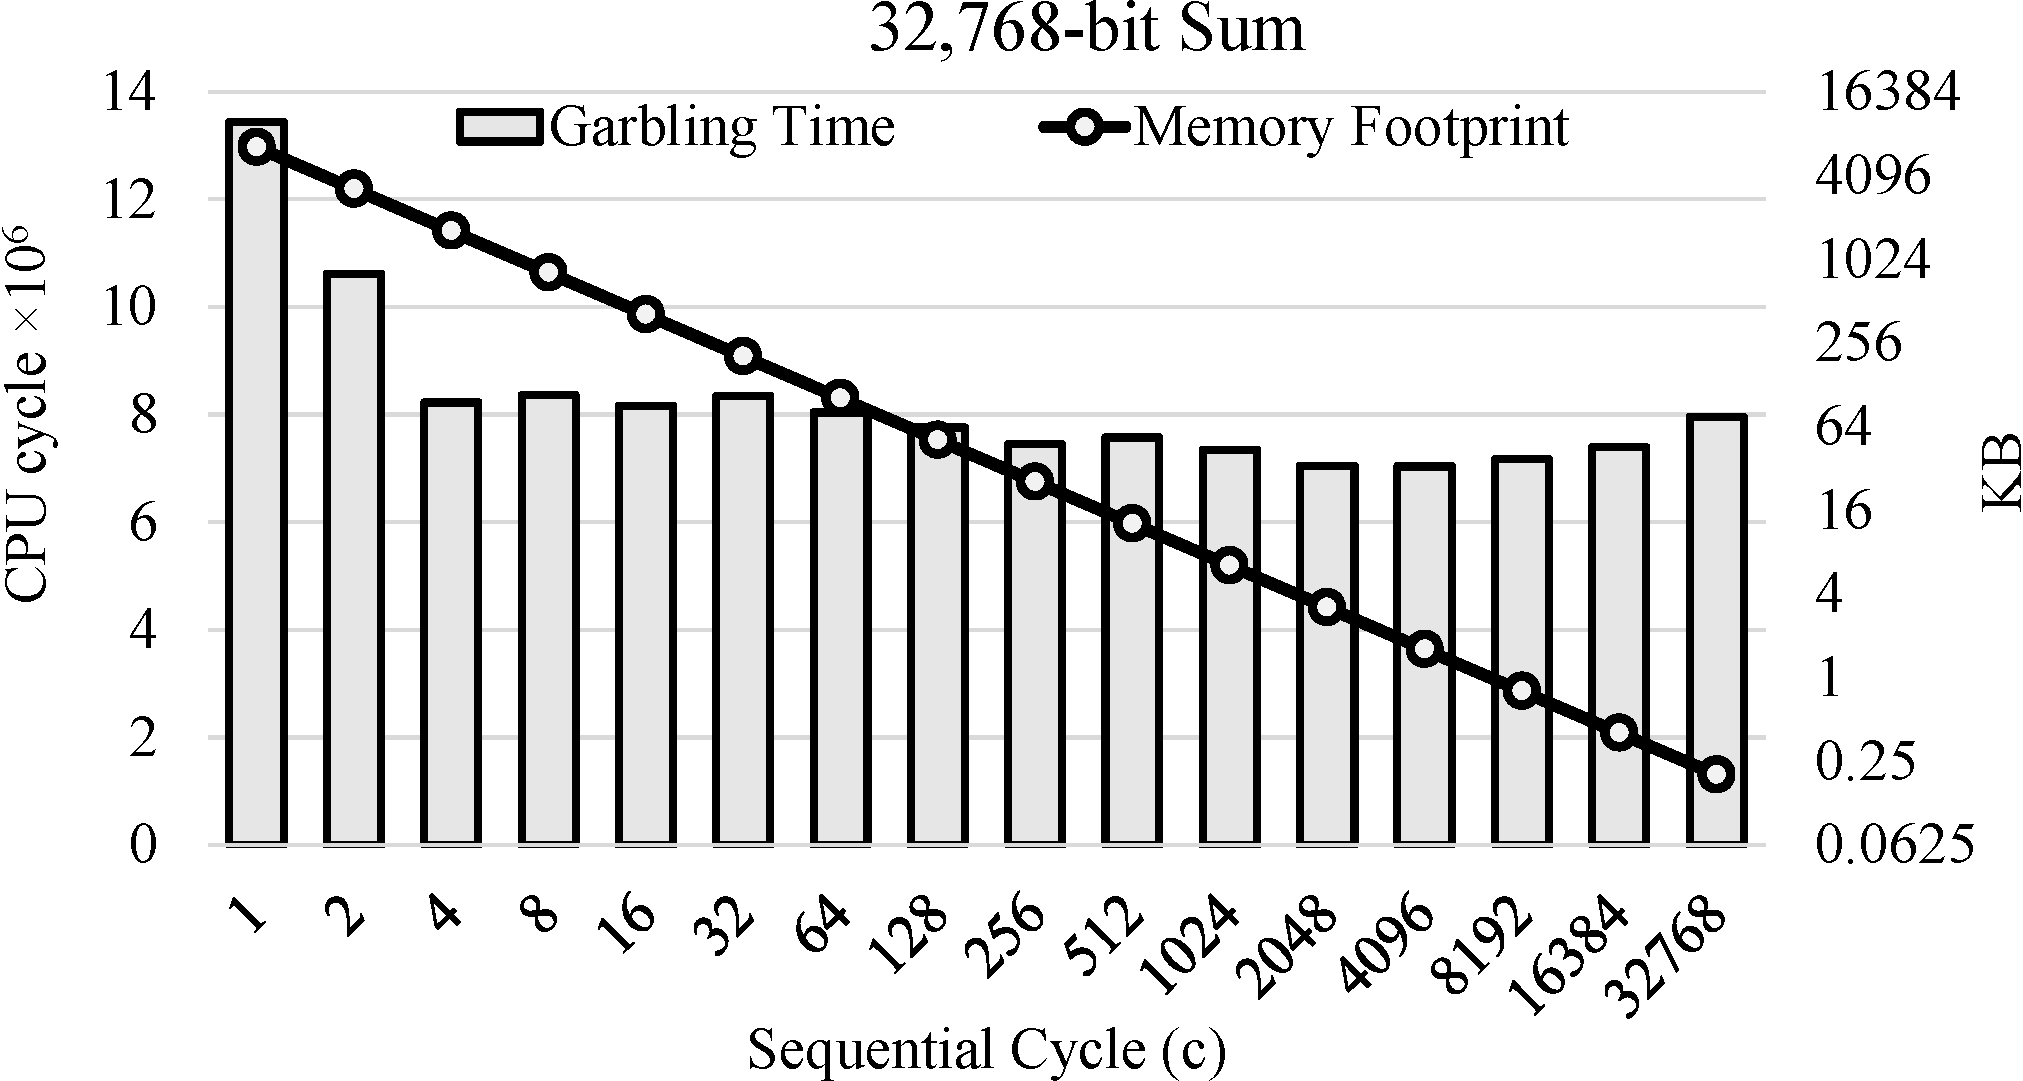
\includegraphics[width=0.9\textwidth]{CPU_Time-crop.pdf}
	\caption{Garbling $\numprint{32768}$-bit Sum function.
The \acrshort{cpu} time in number of cycles and the approximate memory footprint in KBytes (y-axis) versus $cc$ (x-axis) are shown.}
	\label{fig:cpu_time}
\end{figure}

\subsection{high-level Synthesis Tools}\label{ssec:eval-tinygarble-high}
The design automation community has been working on tools that work with higher-level languages and abstractions than \acrshort{hdl}.
While a host of commercial and academic \acrshort{hls} tools are available \cite{tool:Vivado, tool:PandA, decaluwe2004myhdl, Gupta2004}, we selected the Xilinx Vivado \acrshort{hls} for compiling \gls{c} code to \acrshort{hdl} which can then be synthesized using a conventional logic synthesis tool.
The \acrshort{hls} engine in the Vivado suite is built upon the xPilot project \cite{Chapter:Zhang2008}.

\begin{table}
\centering
\caption{Comparison of performance of the circuits generated using \gls{c} input to \acrshort{hls} and a direct \gls{verilog} input to the logic synthesis tool.}
\label{table:hls}
\resizebox{\textwidth}{!}{%
\begin{tabular}{l|r||rr||rr||rr}
\multirow{2}{*}{Function}          & \multicolumn{1}{c||}{\multirow{2}{*}{c}} & \multicolumn{2}{c||}{\gls{c}$\rightarrow$\gls{verilog}}                               & \multicolumn{2}{c||}{\gls{verilog}}                                   & \multicolumn{2}{c}{Comparison}                   \\ \cline{3-8}
                                   & \multicolumn{1}{c||}{}                   & \multicolumn{1}{c}{Non-XOR} & \multicolumn{1}{c||}{Total gates} & \multicolumn{1}{c}{Non-XOR} & \multicolumn{1}{c||}{Total gates} & \multicolumn{1}{c}{\acrshort{mfe}} & \multicolumn{1}{c}{\acrshort{gtd}} \\ \hline \hline
\multirow{3}{*}{16384-bit Compare} & 1,024                                   & 51                          & 70                               & 16                          & 64                               & 0.91                    & 219\%                   \\
                                   & 4,096                                   & 15                          & 21                               & 4                           & 16                               & 0.76                    & 275\%                   \\
                                   & 16,384                                  & 6                           & 9                                & 1                           & 4                                & 0.44                    & 500\%                   \\ \hline
\multirow{3}{*}{160-bit Hamming}   & 1                                       & 1,264                       & 2,142                            & 371                         & 1,230                            & 0.57                    & 241\%                   \\
                                   & 32                                      & 91                          & 146                              & 17                          & 35                               & 0.24                    & 435\%                   \\
                                   & 160                                     & 45                          & 71                               & 10                          & 19                               & 0.27                    & 350\%                   \\ \hline
\multirow{3}{*}{1024-bit Sum}      & 1                                       & 3,067                       & 5,115                            & 1,023                       & 5,114                            & 1.00                    & 200\%                   \\
                                   & 32                                      & 195                         & 292                              & 32                          & 160                              & 0.55                    & 509\%                   \\
                                   & 1,024                                   & 9                           & 11                               & 1                           & 5                                & 0.45                    & 800\%
\end{tabular}
}
\end{table}

\tab{table:hls} demonstrates a comparison between the performance of the circuits generated using \gls{c} input to the \acrshort{hls} tool (\gls{c}$\rightarrow$\gls{verilog}) and a direct \gls{verilog} input.
As can be seen from the table, the resulting memory footprint could increase by a factor between 1 and 4, while the number of garbled tables varies in a range of 3 to 9 times.
It is well known that writing the \acrshort{hdl} level code which contains the time information and more detailed structural/behavioral description would yield much more efficient circuits than the code written in a higher level language.

\section{Evaluation of MIPS for PF-SFE} \label{sec:eval-mips-pf-sfe}
We implement the general purpose processor for \acrshort{pf-sfe} using single-cycle \gls{mips}~I architecture where one user provide function description in assembly and the other provides the data.
Support of sequential circuits in \gls{tinygarble} enables us to use the \gls{mips} circuit description in Plasma project \cite{rhoads2006plasma} without major modifications.
In the following, we provide the result of \gls{mips} implementation and its number of non-XOR and total gates.
Lastly, we present implementation of Hamming distance with variable input length as a benchmark of private function application on \gls{mips}.
More benchmark functions are implemented and their results are compared with \gls{mips} for \gls{sfe} in \sect{sec:eval-mips-sfe}

\subsection{MIPS Implementation}
We used \gls{tinygarble} to generate the \gls{netlist} for the \gls{mips} sequential circuit.
\tab{table:mipsres} shows the total number of gates and non-XOR gates for each module of the \gls{mips} processor with $64\times32$bit DM and IM.
The sum of non-XORs for each module is $\numprint{14997}$.
However, when the modules are combined together to form the entire \gls{mips} processor, the synthesizer optimizes the circuit such that the total number of non-XORs is reduced by $14.95\%$ to $\numprint{12755}$.
The memory footprint for storing labels during garbling \gls{mips} is approximately the size of two labels times the total number of gates which is $2 \times 128 \times \numprint{31719}$bit $=991$~KB for label bit-width $k=128$.
The communication load between parties for invocation of one instruction (one sequential cycle) is approximately the size of two labels times the number of non-XOR gates which is $2\times 128 \times \numprint{12755}$bit $=398$~KB with Half Gate optimization.

\begin{table}
\centering
\caption{Number of total gates and non-XOR gates in the \gls{mips} implementation.
The global optimization of \gls{tinygarble} reduces the overall number of gates compared to that of the sum of individual modules.}\label{table:mipsres}
\begin{tabular}{l|rrl}
Modules             & Total gates & Non-XOR \\ \hline \hline
Controller          & 509                                                  & 470                                                \\
Bus                 & 603                                                  & 590                                                \\
\acrshort{alu}                 & 651                                                  & 346                                                \\
Shifter             & \numprint{1362}                                                 & \numprint{1092}                                               \\
Mult                & \numprint{2147}                                                 & \numprint{1792}                                               \\
Reg File            & \numprint{8880}                                                 & \numprint{3023}                                               \\
\acrshort{im}                  & \numprint{6048}                                                 & \numprint{2016}                                               \\
\acrshort{dm}                  & \numprint{13779}                                                & \numprint{5423}                                               \\
\acrshort{pc}                  & 309                                                  & 245                                                \\ \hline
Total               & \numprint{34288}                                                & \numprint{14997}                                              \\ \hline \hline
\gls{mips}                & \numprint{31719}                                                & \numprint{12755}                                              \\ \hline \hline
\begin{tabular}[c]{@{}l@{}}Global \\optimization\end{tabular} & 7.49\%                                               & 14.95\%
\end{tabular}
\end{table}

\subsection{Benchmark Function}
We implemented the Hamming distance function as a proof-of-concept for our secure \gls{mips} for \acrshort{pf-sfe}.
It counts the number of different elements in two arrays $A$ and $B$ with variable length $l$.
For the hand-optimized assembly code shown in \fig{figure:hamminassembly}, the function requires at most $7+9l$ sequential cycles (instructions) to evaluate.
Thus, based on \tab{table:mipsres}, this function requires overall $\numprint{12755}\times(7+9l)$ non-XOR gates.
It has only $16$ instructions and is stored in $16\times32$bit of the IM.
The function requires that $l$, $A$, and $B$ are stored in addresses $0$, $[2:l+1]$, and $[l+2:2l+1]$ of \acrshort{dm} respectively.
It will store the Hamming distance of $A$ and $B$ in address $1$.


\lstset{
  language=[mips]Assembler,
  escapechar=@, % include LaTeX code between `@' characters
  keepspaces,   % needed to preserve spacing with lstinline
  basicstyle=\footnotesize\ttfamily\bfseries,
  commentstyle=\color{CommentColor},
  stringstyle=\color{cyan},
  showstringspaces=false,
  keywordstyle=[1]\color{blue},    % instructions
  keywordstyle=[2]\color{magenta}, % directives
  keywordstyle=[3]\color{red},     % registers
}

\begin{figure}[ht]
\centering
\resizebox{!}{0.45\textheight}{%
\lstinputlisting{Hamming.s}
}
\caption{Hamming distance assembly code.}\label{figure:hamminassembly}
\end{figure}

\section{Evaluation of MIPS for SFE} \label{sec:eval-mips-sfe}
In this section, we present the evaluation of our approach for high-level \acrshort{sfe} framework using \gls{mips} processor.
We first provide the experimental setup and benchmark function used for evaluating the framework in \sect{sec:eval-mips-sfe-setup} and \sect{ssect:eval-mips-sfe-bench}.
Next, we provide the synthesis result of \gls{mips} processor for various \acrshort{isa}s in \sect{ssect:eval-mips-sfe-isa}.
Lastly, we discuss the performance of our hardware \acrshort{gc} evaluator for the various \acrshort{isa}s and its comparison with the previous work in \sect{ssect:eval-mips-sfe-performance}.

\subsection{Experimental Setup} \label{sec:eval-mips-sfe-setup}
We create different instances of a single-cycle \gls{mips} architecture with specific, restricted, and full \acrshort{isa} to support a trade-off between efficiency and privacy.
The result of full \acrshort{isa} \gls{mips} is presented in previous section (\sect{sec:eval-mips-pf-sfe}) and is used here for comparison.
The different \gls{mips} instances are synthesized using \gls{synopsys-dc} H-2013.03-SP4 to generate optimized sequential Boolean circuits.
These circuits are then evaluated on our hardware \acrshort{gc} evaluator implemented using Vivado 2014.4.1 on a Xilinx Virtex-7 \acrshort{fpga}.

\subsection{Benchmark Function}\label{ssect:eval-mips-sfe-bench}
As benchmark functions, we used Hamming distance, \acrfull{psi}, and \acrshort{aes} functions.
We compile these functions from high-level \gls{c} to \gls{mips} binary using a \gls{mips} cross-compiler.
For some functions, assembly code manipulation allows to reduce the number of sequential cycles required.
To assure correctness of both functions and \acrshort{isa} under test, we simulate the resulting binary file using the Modelsim simulator and calculate the number of required sequential cycles to compute each of the functions, reported in~\tab{tab:cyc_bench}, for accurate performance measurements.
For Hamming distance, the number of cycles depends on the size of the input strings.
In the \acrshort{psi} function, we compute a variant of \acrshort{psi} called \acrfull{psi-ca} where only the number of common elements is revealed.
The sets can have different sizes where each element is 32-bit.
For \acrshort{aes}, we assume that one party holds a 128-bit message and the other party holds eleven round keys each of 128-bit length to avoid unnecessary garbling and evaluation of the round-key generation function.

\begin{table}
\centering
\caption{Number of required cycles to compute the benchmark functions.}\label{tab:cyc_bench}
\begin{tabular}{l||r|r}
\multicolumn{1}{c||}{Function} & \multicolumn{1}{c|}{Input Size} &  \multicolumn{1}{c}{\# of required cycles} \\
\hline
\hline
Hamming distance & $\numprint{16}$ & $\numprint{218}$\\
\hline
 Hamming distance & $\numprint{32}$ & $\numprint{426}$\\
\hline
Hamming distance & $\numprint{64}$ & $\numprint{842}$\\
\hline
Hamming distance & $\numprint{128}$ & $\numprint{1674}$\\
\hline
\acrshort{psi} & $\numprint{64}$ &$\numprint{7267}$\\
\hline
\acrshort{psi} & $\numprint{128}$ &$\numprint{14267}$\\
\hline
\acrshort{aes} (no key expansion) & $\numprint{128}$ & $\numprint{6178}$\\
\end{tabular}
\end{table}

\subsection{Synthesis of MIPS for Various ISAs}\label{ssect:eval-mips-sfe-isa}
We synthesize the \gls{mips} architecture, shown in~\fig{figure:mips}, with \gls{synopsys-dc} for different \acrshort{isa}s and memory sizes: 32 to 512 32-bit words for instruction and data memories.
Generating these Boolean circuits is a one-time process and the circuits can be re-used without incurring further compilation costs.
\tab{tab:synres-app} shows the synthesis time and number of non-XOR gates of the hamming distance-, \acrshort{psi}-, and \acrshort{aes}-specific \acrshort{isa} with different sizes of memories.
\tab{tab:synres-res-full} illustrates the result for restricted and full \acrshort{isa} with different sizes of memories.

\begin{table}
\caption{Synthesis results of application-specific \acrshort{isa}}\label{tab:synres-app}
\centering
\begin{tabular}{l|r|r|r}
\multicolumn{1}{c|}{Memory Size} & \multicolumn{1}{c|}{Synthesis Time} &  \multicolumn{1}{c|}{\# of Combinatorial} & \multicolumn{1}{c}{\# of Sequential} \\
\multicolumn{1}{c|}{(words)} & \multicolumn{1}{c|}{seconds (s)} &  \multicolumn{1}{c|}{non-XOR gates} & \multicolumn{1}{c}{gates} \\
\hline
\hline
\multicolumn{4} {c}{Hamming distance-specific \acrshort{isa}}\\
\hline
\acrshort{dm}, \acrshort{im} = 32 & $\numprint{19.648}$~$s$ & $\numprint{6715}$ & $\numprint{2021}$ \\
\hline
\acrshort{dm}, \acrshort{im} = 64 & $\numprint{31.692}$~$s$ & $\numprint{9830}$ & $\numprint{3046}$ \\
\hline
\acrshort{dm}, \acrshort{im} = 128 & $\numprint{62.212}$~$s$ & $\numprint{16062}$ & $\numprint{5095}$ \\
\hline
\acrshort{dm}, \acrshort{im} = 256 & $\numprint{167.398}$~$s$ & $\numprint{28493}$ & $\numprint{9192}$ \\
\hline
\acrshort{dm}, \acrshort{im} = 512 & $\numprint{589.186}$~$s$ & $\numprint{53374}$ & $\numprint{17385}$ \\
\hline
\multicolumn{4} {c}{\acrshort{psi}-specific \acrshort{isa}}\\
\hline
\acrshort{dm}, \acrshort{im} = 32 & $\numprint{18.735}$~$s$ & $\numprint{6751}$ & $\numprint{2021}$ \\
\hline
\acrshort{dm}, \acrshort{im} = 64 & $\numprint{31.117}$~$s$ & $\numprint{9866}$ & $\numprint{3046}$ \\
\hline
\acrshort{dm}, \acrshort{im} = 128 & $\numprint{61.551}$~$s$ & $\numprint{16097}$ & $\numprint{5095}$ \\
\hline
\acrshort{dm}, \acrshort{im} = 256 & $\numprint{163.564}$~$s$ &$\numprint{28529}$ & $\numprint{9192}$ \\
\hline
\acrshort{dm}, \acrshort{im} = 512 & $\numprint{591.145}$~$s$ & $\numprint{53410}$ & $\numprint{17385}$ \\
\hline
\multicolumn{4} {c}{\acrshort{aes}-specific \acrshort{isa}}\\
\hline
\acrshort{dm}, \acrshort{im} = 256 & $\numprint{169.498}$~$s$ &$\numprint{32177}$ & $\numprint{9214}$ \\
\hline
\acrshort{dm}, \acrshort{im} = 512 & $\numprint{594.047}$~$s$ & $\numprint{61570}$ & $\numprint{17406}$ \\
\end{tabular}
\end{table}

\begin{table}
\caption{Synthesis results of restricted and full \acrshort{isa}}\label{tab:synres-res-full}
\centering
\begin{tabular}{l|r|r|r}
\multicolumn{1}{c|}{Memory Size} & \multicolumn{1}{c|}{Synthesis Time} &  \multicolumn{1}{c|}{\# of Combinatorial} & \multicolumn{1}{c}{\# of Sequential} \\
\multicolumn{1}{c|}{(words)} & \multicolumn{1}{c|}{seconds (s)} &  \multicolumn{1}{c|}{non-XOR gates} & \multicolumn{1}{c}{gates} \\
\hline
\hline
\multicolumn{4} {c}{\acrshort{alu}\&Shift \acrshort{isa}}\\
\hline
\acrshort{dm}, \acrshort{im} = 32 & $\numprint{21.681}$~$s$ & $\numprint{9676}$ & $\numprint{2046}$ \\
\hline
\acrshort{dm}, \acrshort{im} = 64 & $\numprint{34.588}$~$s$ & $\numprint{12702}$ & $\numprint{3070}$ \\
\hline
\acrshort{dm}, \acrshort{im} = 128 & $\numprint{65.873}$~$s$ & $\numprint{19694}$ & $\numprint{5118}$ \\
\hline
\acrshort{dm}, \acrshort{im} = 256 & $\numprint{170.974}$~$s$ &$\numprint{34071}$ & $\numprint{9214}$ \\
\hline
\acrshort{dm}, \acrshort{im} = 512 & $\numprint{593.945}$~$s$ & $\numprint{66238}$ & $\numprint{17406}$ \\
\hline
\multicolumn{4} {c}{\acrshort{alu}-only \acrshort{isa}}\\
\hline
\acrshort{dm}, \acrshort{im} = 32 & $\numprint{19.599}$~$s$ & $\numprint{8136}$ & $\numprint{2046}$ \\
\hline
\acrshort{dm}, \acrshort{im} = 64 & $\numprint{31.970}$~$s$ & $\numprint{11696}$ & $\numprint{3070}$ \\
\hline
\acrshort{dm}, \acrshort{im} = 128 & $\numprint{62.599}$~$s$ & $\numprint{18816}$ & $\numprint{5118}$ \\
\hline
\acrshort{dm}, \acrshort{im} = 256 & $\numprint{164.894}$~$s$ &$\numprint{33041}$ & $\numprint{9214}$ \\
\hline
\acrshort{dm}, \acrshort{im} = 512 & $\numprint{598.986}$~$s$ & $\numprint{65183}$ & $\numprint{17406}$ \\
\hline
\multicolumn{4} {c}{Full \acrshort{isa} (\sect{sec:eval-mips-pf-sfe})}\\
\hline
\acrshort{dm}, \acrshort{im} = 32 & $\numprint{38.331}$~$s$ & $\numprint{13257}$ & $\numprint{2110}$ \\
\hline
\acrshort{dm}, \acrshort{im} = 64 & $\numprint{50.446}$~$s$ & $\numprint{16818}$ & $\numprint{3134}$ \\
\hline
\acrshort{dm}, \acrshort{im} = 128 & $\numprint{82.863}$~$s$ & $\numprint{23899}$ & $\numprint{5182}$ \\
\hline
\acrshort{dm}, \acrshort{im} = 256 & $\numprint{189.157}$~$s$ &$\numprint{38118}$ & $\numprint{9278}$ \\
\hline
\acrshort{dm}, \acrshort{im} = 512 & $\numprint{616.750}$~$s$ & $\numprint{69423}$ & $\numprint{17470}$ \\
\end{tabular}
\end{table}

\begin{itemize}
	\item \emph{Application-specific \acrshort{isa} for public functions:} We synthesized three variants of the application-specific \acrshort{isa} where the selected instructions include only the ones used by a particular function, for various memory sizes.
	We create the application-specific \acrshort{isa} for the three benchmark functions: Hamming distance, \acrshort{psi}, and \acrshort{aes}.
	Instructions required for Hamming distance function are: LW, SW, ADD, SUB, XOR, NOP, SLL and BEQ.
	Instructions required for \acrshort{psi} are: LW, SW, ADD, SUB, NOP, SLL, BEQ, BNE and SLT.
 	Instructions required for \acrshort{aes} areLW, LB, SW, SB, ADD, SUB, AND, XOR, OR, NOP, SLL, SRL, BEQ, BNE, JAL, JR and SLT.

	\item \emph{Restricted \acrshort{isa} for semi-private functions:} We synthesized two variants of the restricted \acrshort{isa}: one without the Mult/Div unit and another without Mult/Div and Shift units.
	Since the difference between the two depends mainly on reducing the control logic and select lines of multiplexers, the numbers of non-XOR gates for both are different.
	However, the number of \acrshort{ff}s are the same.

	\item \emph{Full \acrshort{isa} for private
	functions:} This variant is an extension to the result reported in \sect{sec:eval-mips-pf-sfe} for different memory sizes.
\end{itemize}

\subsection{Performance of the Hardware GC Evaluator} \label{ssect:eval-mips-sfe-performance}
\subsubsection{Area}
\tab{table:resource} shows the resource allocation and utilization of our hardware \acrshort{gc} evaluator on a Xilinx Virtex-7 \acrshort{fpga}.
Note that the \acrshort{fpga} utilization does not vary for different memory sizes and instances of the \gls{mips} processor since the evaluator logic remains unaltered.
For different memory sizes and \acrshort{isa} instances, only the non-XOR gate count varies.
This only impacts the garbled labels and tables memory which significantly affects the off-chip memory utilized for storing the garbled tables, and the \acrfull{bram} resources utilization only to a small extent.

\begin{table}
\centering
\caption{Resource allocation and utilization of our hardware \acrshort{gc} evaluator on a Xilinx Virtex-7 \acrshort{fpga}.}
\label{table:resource}
\begin{tabular}{l|r|r}
Resource    & \multicolumn{1}{c|}{Estimation} & \multicolumn{1}{c}{Utilization \%} \\ \hline \hline
\acrfull{ff} & $\numprint{22035}$ & $\numprint{2.54}$ \\ \hline
Slice \acrfull{lut} & $\numprint{21229}$ & $\numprint{4.90}$ \\ \hline
\acrshort{bram} & $\numprint{354}$ & $\numprint{24}$
\\ \hline
BUFG & $\numprint{2}$ & $\numprint{6.25}$
 \end{tabular}
\end{table}

\subsubsection{Performance}
\tab{table:performance-app} presents the runtime required to evaluate \gls{mips} for one instruction in terms of \acrshort{fpga} clock cycles and $\mu\textrm{s}$ for application-specific \acrshort{isa}s.
\tab{table:performance-res-full} repots the same results for restricted and full \acrshort{isa}s.
Our \acrshort{gc} evaluator operates at $100\textrm{MHz}$ on the \acrshort{fpga}.
This is used to compute an average evaluation runtime of 1.1 \acrshort{fpga} clock cycles per gate for our pipelined \acrshort{gc} evaluator which translates to an average of $11\textrm{ns}$ per gate in our \acrshort{fpga} implementation.
The reported runtime can be further improved by providing tighter timing constraints.

\begin{table}
\centering
\caption{Performance of evaluating \gls{mips} for application-specific \acrshort{isa}s with different memory sizes at $100\textrm{MHz}$ clock frequency on \acrshort{fpga}.}\label{table:performance-app}
\begin{tabular}{l|r|r|r|r|r}
\multicolumn{1}{c|}{Memory Size (words)} & \multicolumn{1}{c|}{$\numprint{32}$ } &  \multicolumn{1}{c|}{$\numprint{64}$ } & \multicolumn{1}{c|}{$\numprint{128}$ } & \multicolumn{1}{c|}{$\numprint{256}$ } & \multicolumn{1}{c}{$\numprint{512}$ }  \\ \hline \hline
\multicolumn{6} {c}{Hamming distance-\acrshort{isa}}\\ \hline
\# of non-XOR gates       & $\numprint{6715}$    & $\numprint{9830}$   & $\numprint{16062}$ & $\numprint{28493}$ & $\numprint{53374}$\\ \hline
Time per inst. (cc)       & $\numprint{7118}$    & $\numprint{10813}$ & $\numprint{17829}$ & $\numprint{30773}$  & $\numprint{57644}$\\ \hline
Time per inst. ($\mu s$) & $\numprint{71.18}$  & $\numprint{108.13}$  & $\numprint{178.29}$  & $\numprint{307.72}$  & $\numprint{576.44}$\\ \hline
Avg. Time per gate (cc)  & $\numprint{1.06}$      & $\numprint{1.10}$   & $\numprint{1.11}$    & $\numprint{1.08}$  & $\numprint{1.08}$\\ \hline
\multicolumn{6} {c}{PSI-\acrshort{isa}}\\ \hline
\# of non-XOR gates       & $\numprint{6751}$    & $\numprint{9866}$   & $\numprint{16097}$ & $\numprint{28529}$ & $\numprint{53410}$\\ \hline
Time per inst. (cc)       & $\numprint{7426}$    & $\numprint{10952}$ & $\numprint{18029}$ & $\numprint{30811}$  & $\numprint{57149}$\\ \hline
Time per inst. ($\mu s$) & $\numprint{74.26}$  & $\numprint{109.52}$  & $\numprint{180.29}$  & $\numprint{308.11}$  & $\numprint{571.49}$\\ \hline
Avg. Time per gate (cc)  & $\numprint{1.10}$      & $\numprint{1.11}$   & $\numprint{1.12}$    & $\numprint{1.08}$  & $\numprint{1.07}$\\ \hline
\multicolumn{6} {c}{\acrshort{aes}-specific \acrshort{isa}}\\ \hline
\# of non-XOR gates       & - & -&- & $\numprint{32177}$   & $\numprint{61570}$\\ \hline
Time per inst. (cc)       &-  & -&- & $\numprint{35717}$   & $\numprint{68343}$\\ \hline
Time per inst. ($\mu s$) & - & -& -& $\numprint{357.17}$ & $\numprint{683.43}$ \\ \hline
Avg. Time per gate (cc)  & -&- &- & $\numprint{1.11}$      & $\numprint{1.11}$ \\
\end{tabular}
\end{table}

\begin{table}
\centering
\caption{Performance of evaluating \gls{mips} for restricted and full \acrshort{isa}s with different memory sizes at $100\textrm{MHz}$ clock frequency on \acrshort{fpga}.}\label{table:performance-res-full}
\begin{tabular}{l|r|r|r|r|r}
\multicolumn{1}{c|}{Memory Size (words)} & \multicolumn{1}{c|}{$\numprint{32}$ } &  \multicolumn{1}{c|}{$\numprint{64}$ } & \multicolumn{1}{c|}{$\numprint{128}$ } & \multicolumn{1}{c|}{$\numprint{256}$ } & \multicolumn{1}{c}{$\numprint{512}$ }  \\ \hline \hline
\multicolumn{6} {c}{ALU\&Shift-\acrshort{isa}}\\
\hline
\# of non-XOR gates       & $\numprint{9676}$    & $\numprint{12702}$ & $\numprint{19694}$ & $\numprint{34071}$  & $\numprint{66238}$\\ \hline
Time per inst. (cc)       & $\numprint{10644}$  & $\numprint{13972}$ & $\numprint{22057}$ & $\numprint{36115}$  & $\numprint{71537}$\\ \hline
Time per inst. ($\mu s$) & $\numprint{106.44}$ & $\numprint{139.72}$  & $\numprint{220.57}$  & $\numprint{361.15}$  & $\numprint{715.37}$\\ \hline
Avg. Time per gate (cc)  & $\numprint{1.10}$     & $\numprint{1.10}$   & $\numprint{1.12}$    & $\numprint{1.06}$  & $\numprint{1.08}$\\ \hline
\multicolumn{6} {c}{ALU-only \acrshort{isa}}\\
\hline
\# of non-XOR gates       & $\numprint{8136}$    & $\numprint{11696}$   & $\numprint{18816}$  & $\numprint{33041}$ & $\numprint{65183}$\\ \hline
Time per inst. (cc)       & $\numprint{8624}$  & $\numprint{12866}$ & $\numprint{21074}$  & $\numprint{35684}$  & $\numprint{73657}$\\ \hline
Time per inst. ($\mu s$) & $\numprint{86.24}$ & $\numprint{128.66}$     & $\numprint{210.74}$  & $\numprint{356.84}$  & $\numprint{736.57}$\\ \hline
Avg. Time per gate (cc)  & $\numprint{1.06}$     & $\numprint{1.10}$    & $\numprint{1.12}$    & $\numprint{1.08}$  & $\numprint{1.13}$\\ \hline
\multicolumn{6} {c}{Full \acrshort{isa} (\sect{sec:eval-mips-pf-sfe})}\\
\hline
\# of non-XOR gates       & $\numprint{13257}$    & $\numprint{16818}$   & $\numprint{23899}$ & $\numprint{38118}$ & $\numprint{69423}$\\ \hline
Time per inst. (cc)       & $\numprint{14848}$  & $\numprint{18668}$ & $\numprint{25811}$ & $\numprint{40786}$  & $\numprint{77060}$\\ \hline
Time per inst. ($\mu s$) & $\numprint{148.48}$ & $\numprint{186.68}$  & $\numprint{258.11}$  & $\numprint{407.86}$  & $\numprint{770.60}$\\ \hline
Avg. Time per gate (cc)  & $\numprint{1.12}$     & $\numprint{1.11}$   & $\numprint{1.08}$    & $\numprint{1.07}$  & $\numprint{1.11}$\\
\end{tabular}
\end{table}

\subsubsection{Comparison with the Prior Art}
\tab{tab:comp} shows a comparison with other \acrshort{gc} evaluator implementations \cite{jarvinen2010garbled, bellare2013efficient}.
However, for fairness, we are leveraging \acrshort{gc} optimizations that were not available at the time for \cite{jarvinen2010garbled}.
We compare with our two implementations, the 21-stage pipelined evaluator and un-pipelined variant to show the effect of pipelining in improving our performance by a factor of 7.8.
\tab{tab:comp} compares our results with interpolated results estimated for other works.
Results indicate that our pipelined \acrshort{gc} evaluator \acrshort{fpga} implementation takes $51\times$ fewer clock cycles compared to the fastest software implementation JustGarble \cite{bellare2013efficient}.
Although the \acrshort{cpu} clock frequency ($3.0\textrm{GHz}$) is $30\times$ faster than that of our Virtex-7 \acrshort{fpga} ($100\textrm{MHz}$), our pipelined implementation would still be almost $2\times$ faster than JustGarble in terms of absolute time.
Note that our implementation is just a prototype on a reconfigurable \acrshort{fpga} as opposed to a custom design of Intel \acrshort{aes-ni} in \acrshort{cpu}.
Implementing our hardware \acrshort{gc} evaluator as ASIC would improve its performance in terms of absolute time even further.
Moreover, our implementation is two orders of magnitude faster than the previously fastest hardware implementation of \cite{jarvinen2010garbled}.

\begin{table}
\centering
\caption{Comparing our \acrshort{gc} evaluator implementation with other works' estimation for \gls{mips} with 64-word memory.}\label{tab:comp}
\begin{tabular}{l||r|r}
\multicolumn{1}{c||}{Method} & \multicolumn{1}{c|}{\begin{tabular}[c]{@{}c@{}}Total time\\(cc)\end{tabular}} & \multicolumn{1}{c}{cc/gate} \\ \hline \hline
J\"arvinen et al. (\acrshort{soc})~\cite{jarvinen2010garbled} & $\numprint{37329233}$ & $\numprint{2219.6}$ \\ \hline
J\"arvinen et al. (Stand-Alone \acrshort{fpga})~\cite{jarvinen2010garbled} & $\numprint{4291954}$ & $\numprint{255.2}$ \\ \hline
JustGarble (\acrshort{cpu})~\cite{bellare2013efficient} & $\numprint{948535}$ & $\numprint{56.4}$ \\ \hline
Our work w/o pipeline & $\numprint{144635}$ & $\numprint{8.6}$ \\ \hline
Our work w/ pipeline & $\numprint{18500}$ & $\numprint{1.1}$
\end{tabular}
\end{table}

% We also compare the overall performance of our \gls{mips} for \acrshot{sfe} with the performance of the proposed software solution in \cite{wang2016secure} on the compatible benchmark functions.
% For computing Hamming distance on two 32-bit integer arrays, Wang et al.'s solution takes $1.24s$ to garble 481K gates (see Table 4 in \cite{wang2016secure}).
% Our solution requires \numprint{6715} non-XOR gates and \numprint{426} cycles (see Tables \ref{tab:synres} and \ref{tab:cyc_bench}), and thus it takes only $0.0314s$ to evaluate 2.8M gates.
% Given that garbling time is double the evaluation time, this indicates a speedup of factor 18 for our solution but with $6\times$ more non-XOR gates for the same functionality.
% In terms of throughput, our approach can evaluate 90.8M gates and Wang et al.'s solution can evaluate 776K gates which makes ours 117 times faster owing to our hardware implementation.
% However, this speedup assumes on-chip memory and is likely to be much smaller when utilizing off-chip memory.

\section{Evaluation of ARM2GC}\label{sec:eval-arm2gc}
In this section, we present the evaluation result of the \gls{skipgate} algorithm and the \gls{arm2gc} framework.
First, we explain the experimental setup of the evaluation.
Next, the effect of the \gls{skipgate} algorithm on removing sequential overhead from the benchmark function is reported.
We then compare the result of the \gls{arm2gc} framework and that of \gls{tinygarble} \acrshort{gc} synthesis and high-level custom compiler approaches of the previous work.
The effect of the \gls{skipgate} algorithm on the \gls{arm} circuit is illustrated next.
Lastly, we provide a number of complex functions that has been implemented using the \gls{arm2gc} framework.

\subsection{Experimental Setup}
We use \gls{synopsys-dc} H-2013.03-SP4~\cite{tool:DesignCompiler} along with \gls{tinygarble} synthesis flow and technology libraries to generate the \gls{netlist}s for the benchmark circuits and the \gls{arm} processor.

For the \gls{arm2gc} framework, we use the Amber \gls{arm} project, an open-source implementation of \gls{arm} v2a \acrshort{isa} on opencores~\cite{santifort2010amber}.
The \gls{arm} circuit is modified as explained in \sect{ssec:arm}.
Synthesizing the \gls{arm} processor with \gls{synopsys-dc} takes few hours.
However, the process is done only once for a given memory size and it can be used for any set of functions and inputs afterwards.
The benchmark functions for \gls{arm2gc} are implemented in \gls{c} and compiled using GNU gcc-arm-linux-gnueabi (Ubuntu/Linaro 5.3.1-14ubuntu2).
We used \texttt{-Os} compiler optimization flag in order to reduce the number of instructions.
We modified the header assembly code to change the addresses of stack, code, and data memories in the compiled binary.
We do not apply any optimization on the binary code.
Thus, similar to a normal software compilation, it takes less than a few seconds to compile a function into an \gls{arm} binary code.

\subsection{Effect of {SkipGate} on Sequential GC}
As described in \chap{chap:skipgate}, the \gls{skipgate} algorithm avoids redundant garbling/evaluation of gates in sequential circuits with public wires.
In the sequential benchmark circuits reported in \sect{ssec:eval-tinygarble-seq} for \gls{tinygarble} sequential synthesis, the flip-flops were initialized with known values but their output wires were treated as secret.
We applied \gls{skipgate} to the same benchmark functions to demonstrate the cost reduction even for small number of public values.
In \tab{tab:sys_impvoment}, we compare the cost of garbling for circuits generated by \gls{tinygarble} with and without applying the \gls{skipgate} algorithm.
The results without \gls{skipgate} are the same as the ones in second and third columns of \tab{table:result-seq} in \sect{ssec:eval-tinygarble-seq}.
The total number of non-XOR gates to be garbled is cc$\times$\#non-XORs in the sequential circuit and is shown in the second column.
The table also reports the cost of garbling of the same circuits by employing the \gls{skipgate} algorithm (third column) and their percentage improvement (fifth column).
As can be seen, cost reduction of \gls{skipgate} can be as high as $59.5\%$ for \acrshort{aes} and as little as $0\%$ in Compare function.

The degree of improvement depends on the structure of the circuit and whether or not the registers are connected to non-XOR gates.
For example in \acrshort{aes}, garbling of the controller part of the sequential circuit (including a counter keeping track of the \acrshort{aes} round and \acrshort{mux}s connecting to it) is avoided by \gls{skipgate} because both parties know the \acrshort{aes} control path in advance.
Note that the functions in \tab{tab:sys_impvoment} do not have any public known inputs that are the main target of \gls{skipgate}.
Nevertheless, \gls{skipgate} reduces the cost of \acrshort{gc} by leveraging the public initial value of the small number of flip-flops in the functions.

\begin{table}
\centering
\caption{\gls{skipgate} algorithm improvement on sequential circuits generated by \acrfull{tg} synthesis flow (\sect{ssec:eval-tinygarble-seq}).
	These functions do not have public inputs.
	\gls{skipgate} benefits from the small number of flip-flops initial values that are public to reduce their garbling cost.}\label{tab:sys_impvoment}
\begin{tabular}{l||r|r|r||r}
\multirow{2}{*}{Function (bit)} & \multicolumn{2}{c|}{\# of garbled non-XOR} & \multicolumn{1}{c||}{\multirow{2}{*}{\begin{tabular}[c]{@{}c@{}}\# of skipped\\ non-XOR\end{tabular}}} & \multicolumn{1}{c}{\multirow{2}{*}{Improv.}} \\ \cline{2-3}
 & \multicolumn{1}{c|}{\acrshort{tg}~(\sect{ssec:eval-tinygarble-seq})} & \multicolumn{1}{c|}{\gls{skipgate}} & \multicolumn{1}{c||}{} & \multicolumn{1}{c}{} \\ \hline \hline
Sum 32 & 32 & 31 & 1 & 3.1\% \\
Sum 1024 & 1,024 & 1,023 & 1 & 0.1\% \\ \hline
Compare 32 & 32 & 32 & 0 & 0.0\% \\
Compare 16,384 & 16,384 & 16,384 & 0 & 0.0\% \\ \hline
Hamming 32 & 160 & 145 & 15 & 9.4\% \\
Hamming 160 & 1,120 & 1,092 & 28 & 2.5\% \\
Hamming 512 & 4,608 & 4,563 & 45 & 1.0\% \\ \hline
Mult 32 & 2,048 & 2,016 & 32 & 1.6\% \\ \hline
MatrixMult3x3 32 & 25,947 & 25,668 & 279 & 1.1\% \\
MatrixMult5x5 32 & 120,125 & 119,350 & 775 & 0.6\% \\
MatrixMult8x8 32 & 492,032 & 490,048 & 1,984 & 0.4\% \\ \hline
\acrshort{aes} 128$\dagger$ & 15,807 & 6,400 & 9,407 & 59.5\% \\ \hline
\acrshort{sha}3 256 & 40,032 & 38,400 & 1,632 & 4.1\%
\end{tabular}
\\
\footnotesize{{$\dagger$}The missing key expansion module to \acrshort{aes} 128 of \tab{table:result-seq} in \sect{ssec:eval-tinygarble-seq} is added here.}
\end{table}

\subsection{ARM2GC vs Logic Synthesis}
\tab{table:hw_vs_frwk} compares the cost of garbling of functions devised in \gls{verilog} \acrshort{hdl} and constructed by the hardware synthesis technique of \gls{tinygarble} \acrshort{gc} synthesis (see \chap{chap:syn}) with functions developed in \gls{c} and constructed by the \gls{arm2gc} framework.
The results of \gls{tinygarble} \acrshort{gc} synthesis are repeated here from \tab{table:result-comb} in \sect{ssec:eval-tinygarble-comb} for comparison.
As expected, \gls{arm2gc} incurs only a small overhead (at most 6.2\% for MatrixMult8x8) compared to  hardware synthesis method.
In case of Hamming distance function, \gls{arm2gc} results in even less number of non-XOR gates (up to $78\%$ improvement).
Note that we use an efficient binary tree-based method~\cite{huang2011faster} for Hamming distance realization in \gls{c}.

\begin{table}
\centering
\caption{The number of garbled non-XOR gates for the benchmark functions. Comparing \gls{arm2gc} to \gls{tinygarble}'s \acrshort{gc} synthesis (\chap{chap:syn}).}\label{table:hw_vs_frwk}
\begin{tabular}{l||r|r||r}
Function (bit) & \multicolumn{1}{c|}{\begin{tabular}[c]{@{}c@{}}\gls{tinygarble}\\ (\gls{verilog})~(\sect{ssec:eval-tinygarble-comb})\end{tabular}} & \multicolumn{1}{c||}{\begin{tabular}[c]{@{}c@{}}\gls{arm2gc}\\ (\gls{c})\end{tabular}} & \multicolumn{1}{c}{Overhead} \\ \hline \hline
Sum 32 & 31 & 31 & 0.0\% \\
Sum 1024 & 1,023 & 1,023 & 0.0\% \\ \hline
Compare 32 & 32 & 32 & 0.0\% \\
Compare 16,384 & 16,384 & 16,384 & 0.0\% \\ \hline
Hamming 32 & 160 & 57 & -64.4\% \\
Hamming 160 & 1,120 & 247 & -77.9\% \\
Hamming 512 & 4,608 & 1,012 & -78.0\% \\ \hline
Mult 32 & 1,023 & 993 & -2.9\% \\ \hline
MatrixMult3x3 32 & 27,369 & 27,369 & 0.0\% \\
MatrixMult5x5 32 & 120,125 & 127,225 & 5.9\% \\
MatrixMult8x8 32 & 492,032 & 522,304 & 6.2\% \\ \hline
\acrshort{aes} 128$\dagger$ & 6,400 & 6,400 & 0.0\% \\ \hline
\acrshort{sha}3 256 & 38,400 & 37,760 & -1.7\% \\
\end{tabular}
\\
\footnotesize{{$\dagger$}The missing key expansion module to \acrshort{aes} 128 of \tab{table:result-comb} in \sect{ssec:eval-tinygarble-comb} is added here.}
\end{table}

\subsection{ARM2GC vs GC Frameworks Supporting High-level Languages}
\tab{table:other_compiler_vs_frwk} reports the cost of garbling for the benchmark functions constructed by the prior-art \acrshort{gc} frameworks including (\gls{tinygarble} \acrshort{hls} synthesis in \chap{chap:syn} and \cite{holzer2012secure, mood2016frigate}).
\tab{table:other_processor_vs_frwk} reports the comparison with previous work on garbled processors approaches (\gls{mips} for \acrshort{pf-sfe} in \sect{sec:processor-pfsfe} and for \acrshort{sfe} in \sect{sec:processor-mips-sfe} and \cite{wang2016secure}).
The corresponding programming language is shown between parentheses.
Note that this is not an exhaustive list and only includes the most recent \acrshort{gc} frameworks that report the best results on the benchmark functions.
In all cases, \gls{arm2gc} outperforms the earlier frameworks in terms of garbling cost.
For example, \gls{arm2gc} results $12.2\times$,  $5.1\times$, $74,000\times$, $57,000\times$, and $2.9\times$ less number of non-XOR gates for 160-bit Hamming distance compared to \acrshort{ansi}-\gls{c}~\cite{holzer2012secure}, \gls{tinygarble} \acrshort{hls} approach (\sect{ssec:eval-tinygarble-high}), \acrshort{pf-sfe} \gls{mips} (\sect{sec:eval-mips-pf-sfe}), \acrshort{sfe} \gls{mips} (\sect{sec:eval-mips-sfe} and \cite{wang2016secure}), and \gls{frigate}~\cite{mood2016frigate} respectively.
\gls{arm2gc} also results in $38.3\%$ less non-XOR gates compared to \gls{frigate}~\cite{mood2016frigate} for \acrshort{aes} function.

\begin{table}
\centering
\caption{Number of garbled non-XOR gates for the benchmark functions.
Comparing \gls{arm2gc} with previous high-level custom compiler methods and \gls{tinygarble} \acrshort{hls} approach.}
\label{table:other_compiler_vs_frwk}
\begin{tabular}{l||r|r|r||r}
Function (bit) & \begin{tabular}[c]{@{}l@{}}\acrshort{ansi}-\gls{c}\\ (\gls{c}) \\ \cite{holzer2012secure}\end{tabular} & \begin{tabular}[c]{@{}l@{}}\acrshort{tg} \acrshort{hls}\\ (\gls{c} $\rightarrow$ \gls{verilog}) \\ (\sect{ssec:eval-tinygarble-high})\end{tabular} & \begin{tabular}[c]{@{}l@{}}Frigate\\ (\gls{c})\\ \cite{mood2016frigate}\end{tabular} & \begin{tabular}[c]{@{}l@{}}ARM2GC\\ (\gls{c})\end{tabular} \\ \hline \hline
Sum 32           & 32                                                   & 288                                                            & -                                                     & 31                                                   \\
Sum 1024         & -                                                    & 9,216                                                          & 1,025                                                 & 1,023                                                \\ \hline
Compare 32       & 65                                                   & 102                                                            & -                                                     & 32                                                   \\
Compare 16,384   & -                                                    & 52,224                                                         & 16,386                                                & 16,384                                               \\ \hline
Hamming 32       & 601                                                  & 253                                                            & -                                                     & 57                                                   \\
Hamming 160      & 3,003                                                & 1,264                                                          & 719                                                   & 247                                                  \\
Hamming 512      & 9,610                                                & 4,045                                                          & -                                                     & 1,012                                                \\ \hline
Mult 32          & 1,741                                                & -                                                              & 995                                                   & 993                                                  \\ \hline
MatrixMult3x3 32 & 47,583                                               & -                                                              & -                                                     & 27,369                                               \\
MatrixMult5x5 32 & 220,825                                              & -                                                              & 128,252                                               & 127,225                                              \\
MatrixMult8x8 32 & 905,728                                              & -                                                              & -                                                     & 522,304                                              \\ \hline
\acrshort{sha}3 256         & -                                                    & -                                                              & -                                                     & 37,760                                               \\ \hline
\acrshort{aes} 128          & -                                                    & -                                                              & 10,383                                                & 6,400
\end{tabular}
\end{table}

\begin{table}
\centering
\caption{Number of garbled non-XOR gates for the benchmark functions.
Comparing \gls{arm2gc} with the previous garbled processor approaches.}
\label{table:other_processor_vs_frwk}
\begin{tabular}{l||r|r|r||r}
Function (bit)   & \begin{tabular}[c]{@{}l@{}}\acrshort{pf-sfe} \gls{mips}\\ (\gls{c})\\ (\sect{sec:eval-mips-pf-sfe})\end{tabular} & \begin{tabular}[c]{@{}l@{}}\acrshort{sfe} \gls{mips}\\ (\gls{c})\\ \cite{wang2016secure}\end{tabular} & \begin{tabular}[c]{@{}l@{}}\acrshort{sfe} \gls{mips}\\ (\gls{c})\\ (\sect{sec:eval-mips-sfe})\end{tabular} & \begin{tabular}[c]{@{}l@{}}\gls{arm2gc}\\ (\gls{c})\end{tabular} \\ \hline \hline
Sum 32           & -                                                         & -                                                      & -                                                                & 31                                                   \\
Sum 1024         & -                                                         & -                                                      & -                                                                & 1,023                                                \\ \hline
Compare 32       & -                                                         &                                                        & -                                                                & 32                                                   \\
Compare 16,384   & -                                                         & -                                                      & -                                                                & 16,384                                               \\ \hline
Hamming 32       & 3,762,725                                                 & 481,000                                                & 2,860,590                                                        & 57                                                   \\
Hamming 160      & 18,456,485                                                & -                                                      & 14,302,950                                                       & 247                                                  \\
Hamming 512      & 58,864,325                                                & 49,600,000                                             & 45,769,440                                                       & 1,012                                                \\ \hline
Mult 32          & -                                                         & -                                                      & -                                                                & 993                                                  \\ \hline
MatrixMult3x3 32 & -                                                         & -                                                      & -                                                                & 27,369                                               \\
MatrixMult5x5 32 & -                                                         & -                                                      & -                                                                & 127,225                                              \\
MatrixMult8x8 32 & -                                                         & -                                                      & -                                                                & 522,304                                              \\ \hline
\acrshort{sha}3 256         & -                                                         & -                                                      & -                                                                & 37,760                                               \\ \hline
\acrshort{aes} 128          & -                                                         & -                                                      & 198,789,506                                                      & 6,400
\end{tabular}
\end{table}

\subsection{Effect of {SkipGate} on ARM}
\tab{tab:sys_improvment_frwk} shows the cost of garbling an \gls{arm} processor for the benchmark functions using conventional \acrshort{gc} compared to \acrshort{gc} with the \gls{skipgate} algorithm.
Since the instruction memory is known to both parties in \gls{arm}, \gls{skipgate} omits a significant number of non-XOR gates in the circuits.
The circuit of \gls{arm} has 126,755 non-XOR gates and for computing a function, for example Hamming 160, it takes 1,909 sequential cycles.
It means with the conventional \acrshort{gc} protocol, garbling/evaluation of $1,909\times126,755=241,975,295$ non-XORs is required.
While \gls{skipgate} reduces the circuit into a smaller circuit with only 247 non-XORs (almost 7 orders of magnitude less).
In the case of \acrshort{aes}, we achieve more than {\it six orders of magnitude} improvement over the conventional \acrshort{gc} without the \gls{skipgate} algorithm.
The algorithm transforms the impracticable cost of garbling an \gls{arm} processor into near-optimal cost of the reduced circuit.
These dramatic improvements are due to the large number of public inputs in the \gls{arm} processor that allows \gls{skipgate} to skip garbling/evaluation most of the non-XOR gates in the \gls{arm} circuit.

\begin{table}
\centering
\caption{\gls{skipgate} algorithm improvement on the \gls{arm} sequential circuit.}
\label{tab:sys_improvment_frwk}
\begin{tabular}{l||r|r||r}
\multirow{2}{*}{Function (bit)} & \multicolumn{2}{c||}{\# of non-XOR gates} &
\multicolumn{1}{c}{\multirow{2}{*}{\begin{tabular}[c]{@{}c@{}}Improvement \\ (1000X)\end{tabular}}} \\ \cline{2-3}
& \multicolumn{1}{c|}{Conventional \acrshort{gc}+\gls{arm}} & \multicolumn{1}{c||}{\gls{arm2gc}} & \multicolumn{1}{c}{} \\ \hline
Sum 32 & 3,817,680 & 31 & 123 \\
Sum 1024 & 76,483,260 & 1,023 & 75 \\
Compare 32 & 4,072,192 & 130 & 31 \\
Compare 16,384 & 1,047,095,280 & 16,384 & 64 \\
Hamming 32 & 67,063,912 & 57 & 1,177 \\
Hamming 160 & 242,931,704 & 247 & 984 \\
Hamming 512 & 863,559,216 & 1,012 & 853 \\
Mult 32 & 4,199,448 & 993 & 4 \\
MatrixMult3x3 32 & 72,790,432 & 27,369 & 3 \\
MatrixMult5x5 32 & 286,071,488 & 127,225 & 2 \\
MatrixMult8x8 32 & 1,079,894,416 & 522,304 & 2 \\
\acrshort{sha}3 256 & 29,354,783,052 & 37,760 & 777 \\
\acrshort{aes} 128 & 54,621,701,856 & 6,400 & 8,535
\end{tabular}
\end{table}

Comparing the result of \tab{tab:sys_impvoment} and \tab{tab:sys_improvment_frwk} shows that the extend of \gls{skipgate}'s impact highly depends on the structure of the circuit, as well as the degree of presence of public values in the circuit.

\subsection{Complex Functions}
As shown in \tab{tab:complex_funct}, we also develop a number of more complex functions with the \gls{arm2gc} framework.

\begin{table}
\centering
\caption{\gls{skipgate} algorithm improvement on the \gls{arm} sequential circuit for the complex functions.}
\label{tab:complex_funct}
\begin{tabular}{l||r|r||r}
\multirow{2}{*}{Function (bit)} & \multicolumn{2}{c||}{\# of non-XOR gates} & \multicolumn{1}{c}{\multirow{2}{*}{\begin{tabular}[c]{@{}c@{}}Improvement \\ (1000X)\end{tabular}}} \\ \cline{2-3}
 & \multicolumn{1}{c|}{Conventional \acrshort{gc}+\gls{arm}} & \multicolumn{1}{c||}{\gls{arm2gc}} & \multicolumn{1}{c}{} \\ \hline
Bubble-Sort32 32 & 1,366,390,620 & 65,472 & 21 \\
Merge-Sort32 32 & 981,712,458 & 540,645 & 2 \\
Dijkstra64 32 & 1,493,339,886 & 59,282 & 25 \\
\acrshort{cordic} 32 & 228,847,596 & 4,601 & 50
\end{tabular}
\end{table}

\subsubsection{Bubble-Sort32}
This function receives a list of 32 32-bit integers, sorts the list using Bubble Sort algorithm, and then writes the sorted list on the output memory.

\subsubsection{Merge-Sort32}
This function receives a list of 32 32-bit integers, sorts the list using Merge Sort algorithm, and then writes the sorted list on the output memory.

\subsubsection{Dijkstra}
This function receives the adjacency matrix of a directed graph with 64 weighted edges (described as 32-bit integer), finds the shortest path between a source and other nodes using Dijkstra algorithm, and then writes the corresponding distances in the output memory.

\subsubsection{CORDIC}
\acrfull{cordic} function receives a degree and a 2D vector described as 32-bit fixed-point (2-bit decimal and 30-bit fraction), computes trigonometric, hyperbolic or exponential functions according to Universal \acrshort{cordic} algorithm~\cite{volder1959cordic}, and then writes the final 2D vector on the output memory.
The output vector in \acrshort{cordic} algorithm converges one bit per iteration thus, it requires 32 iterations in our case.
The only required operations are addition, shift, and non-oblivious table lookup.
Universal \acrshort{cordic} has two modes for updating vector: rotational and vectoring and three modes for lookup table: circular, linear, and hyperbolic.
Combining these two modes allows user to compute trigonometric, hyperbolic, exponential, square-root, multiplication, or division functions in each combination.
Among these functions square-root and division have previously been reported in~\cite{hussain2016privacy} and required $12,733$ and $12,546$ non-XOR gates respectively, almost three times more than \gls{arm2gc}.
